\documentclass{beamer}

% packages
\usepackage[slovak]{babel}
\usepackage[utf8]{inputenc}
\usepackage[T1]{fontenc}

% theme
\usetheme{metropolis}
\setbeamertemplate{footline}[frame number]

% title
\title{Lúštenie historických šifier na GRIDe}
\author{Bc. Martin Eliáš}
\date{Ing. Eugen Antal, PhD.}
\institute{Slovenská technická univerzita v Bratislave}

\begin{document}
\maketitle

% vacsi doraz na vypoctovu techniku
\begin{frame}{Úvod}
  \begin{itemize}
  \item Historické šifry
  \item Grid vrámci STU
  \item Monoalfabetická substitúcia
  \item Paralelné genetické algoritmy
  \end{itemize}
\end{frame}

% zdoraznit univerzalnost a buduce vyuzitie, zjednodusenie prace
\begin{frame}{Požiadavky}
  \begin{itemize}
  \item Automatické vytváranie projektov
  \item Lokálny vývoj a testovanie
  \item Zdieľanie modulov medzi projektami
  \item Automatické generovanie a úprava skriptov pre gridové prostredie
  \item Jednoduchá synchronizácia s gridom hpc.stuba.sk
  \end{itemize}
\end{frame}

\begin{frame}{Príklad použitia}
  \begin{figure}
    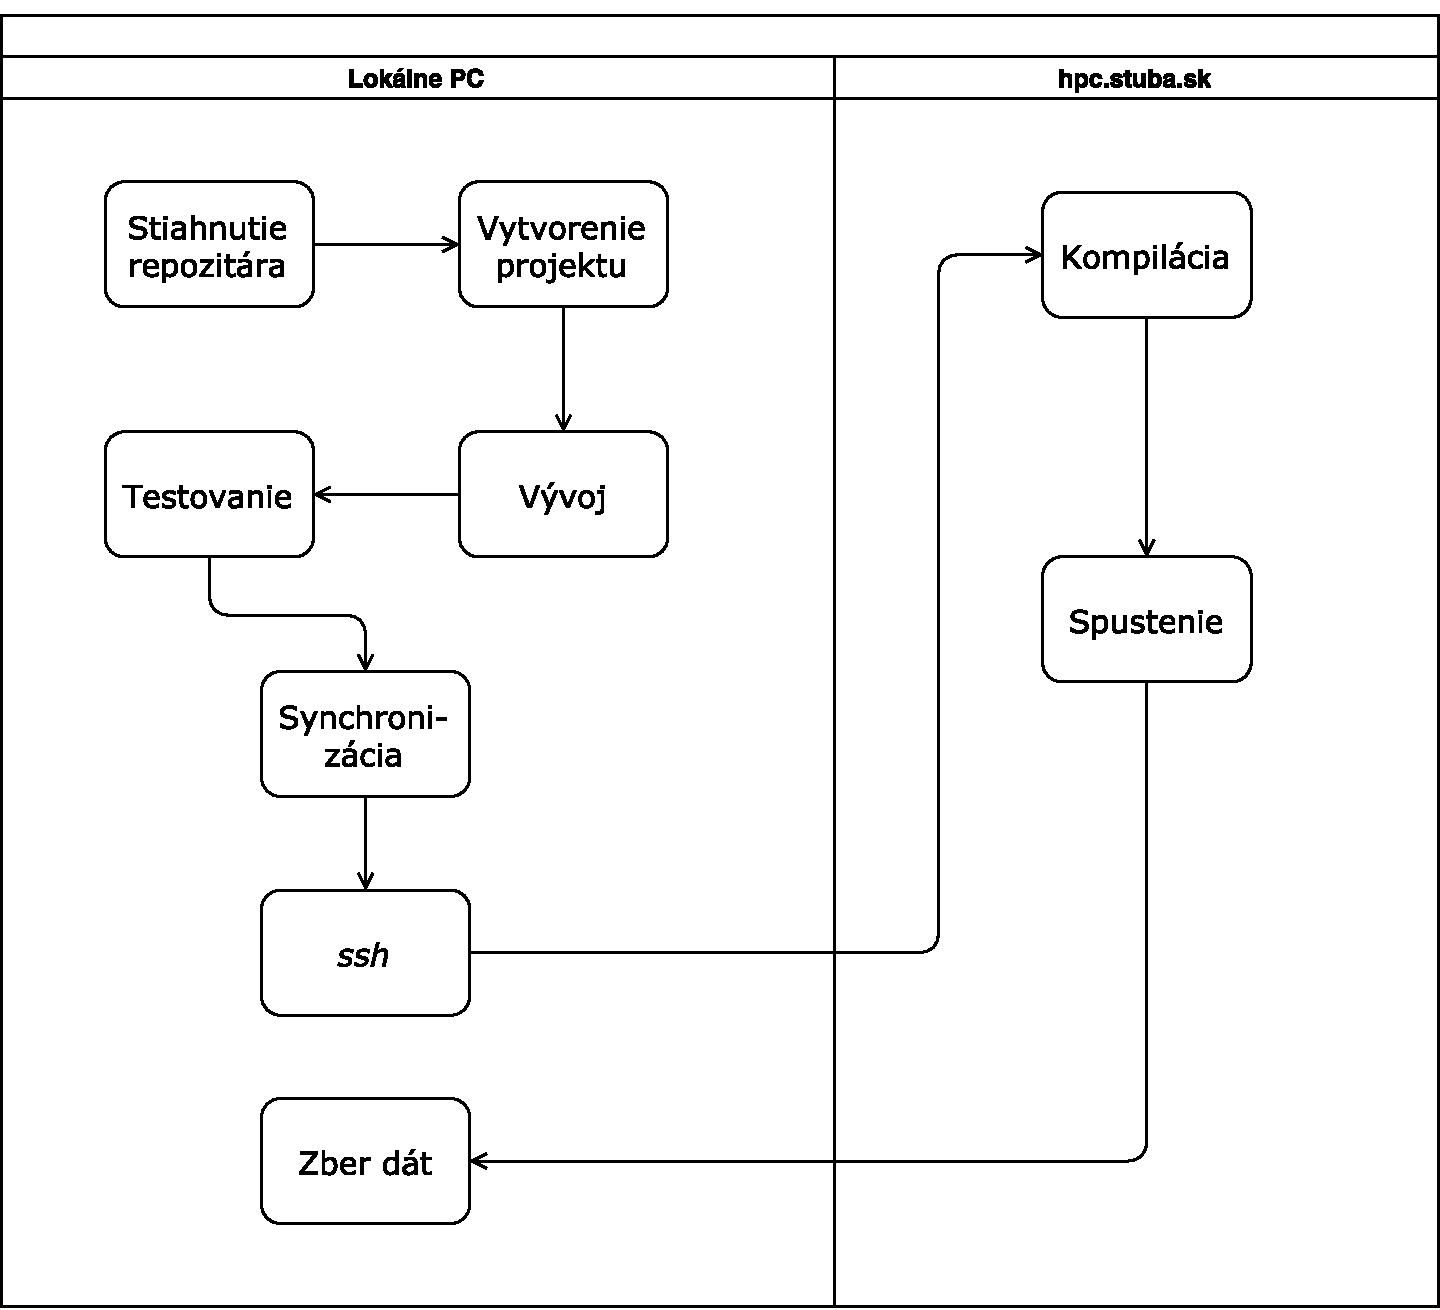
\includegraphics[scale=0.35]{img/uc.pdf}
  \end{figure}
\end{frame}

\begin{frame}{Technológie}
  \begin{itemize}
  \item C++
  \item CMake
  \item Boost
  \item MPI
  \item Git
  \end{itemize}
\end{frame}

\begin{frame}{build.sh}
  \begin{itemize}
  \item Vytvorenie projektu
  \item Kompilácia
  \item Spúštanie projektov
  \item Synchronizácia s gridom
  \end{itemize}
\end{frame}

\begin{frame}{Genetické algoritmy}
  \begin{itemize}
  \item Implementácia
  \item Vytváranie schém
  \item Distribúcia parametrov
  \end{itemize}
\end{frame}

% skumame vplyv parametrov na uspesnost lustenia
\begin{frame}{Experiment s GA}
  \begin{itemize}
  \item Veľkosť populácie: 10, 20, 50, 100
  \item Počet iterácií: 10000, 50000
  \item 10 rôznych schém
  \item Dĺžky textov od 50, 100, ..., 2000
  \item 34 hodín, 320 000 spustení GA
  \end{itemize}
\end{frame}

\begin{frame}{Výsledky GA 50000 iterácií 100 jedincov}
  \begin{figure}
    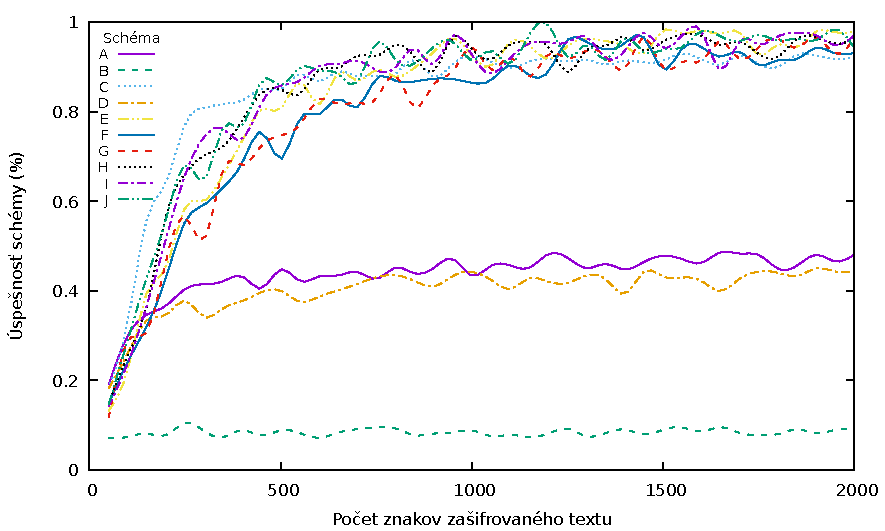
\includegraphics[scale=0.75]{img/GA_50000_100.pdf}
  \end{figure}
\end{frame}

\begin{frame}{Výsledky GA 50000 iterácií 100 jedincov}
  \begin{figure}
    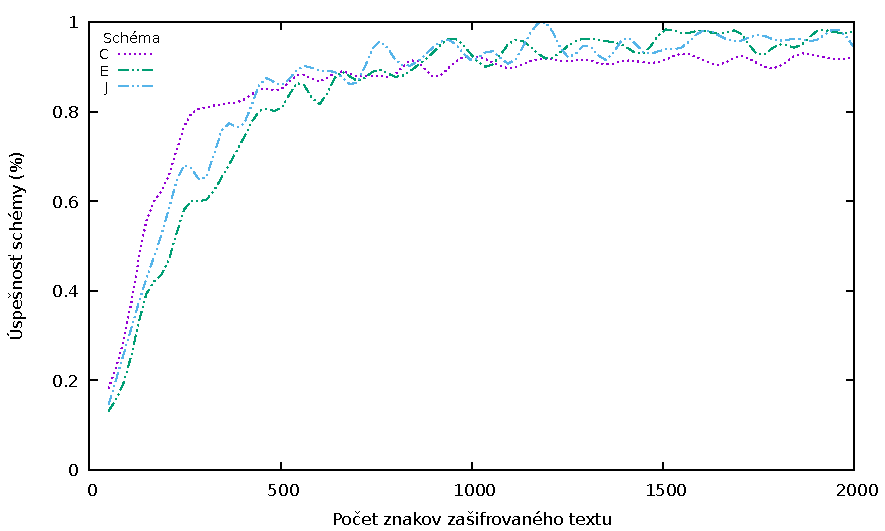
\includegraphics[scale=0.75]{img/GA_CEJ_50000_100.pdf}
  \end{figure}
\end{frame}

% pga premostenie z ga
% pga je vviac ga ktore si vymienaju info
% povedat kratko nieco k topologii
\begin{frame}{Experiment s PGA}
  \begin{itemize}
  \item 3 schémy z predchádzajúceho exprimentu
  \item 4 rôzne topológie
  \item Veľkosti topológií: 3, 5, 11
  \item Migračný čas: 1000, 5000, 10000 iterácií
  \item 2,5 týždňa, viac ako 7 000 000 spustení GA
  \end{itemize}
\end{frame}

\begin{frame}{Toplógie PGA}
  \begin{figure}
    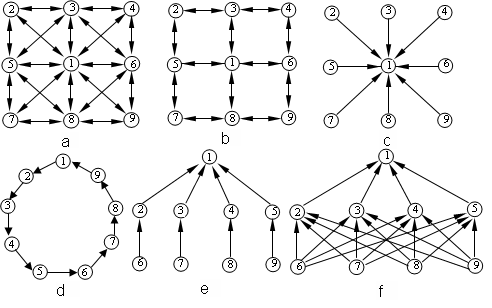
\includegraphics[scale=0.5]{img/topology.png}
  \end{figure}  
\end{frame}

\begin{frame}{Výsledky PGA}
  \begin{figure}
    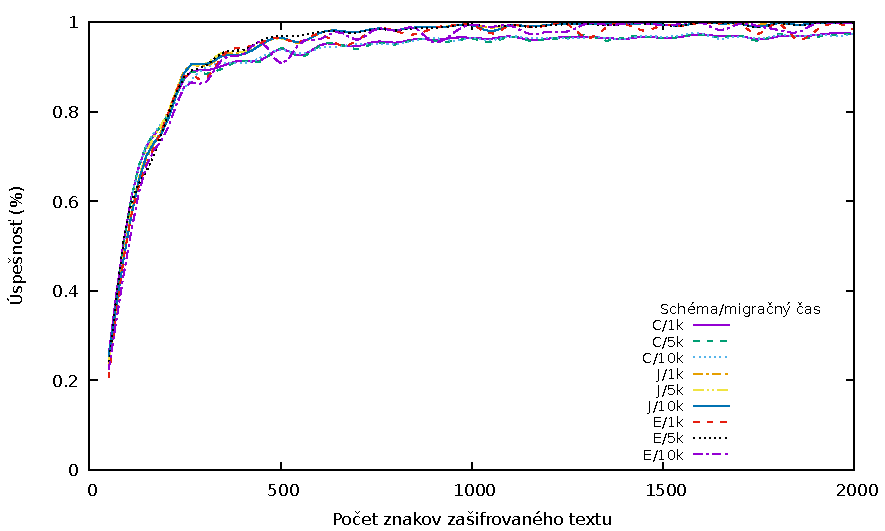
\includegraphics[scale=0.75]{img/PGA.pdf}
  \end{figure}  
\end{frame}

\begin{frame}{Zhrnutie}
  \begin{itemize}
  \item Vytvorenie nástrojov na kryptoanalýzu
  \item Modul PGA
  \item Vplyv veľkosti populácie na úspešnosť
  \item Takmer 100\% úspešnosť riešenia pri PGA
  \item Možné využitie pre ďalších riešiteľov
  \end{itemize}
\end{frame}

\section{Ďakujem za pozornosť}

\begin{frame}{Oponentská otázka}
  \begin{itemize}
  \item Čo je to manhatanovská vzdialenosť?
  \end{itemize}
\end{frame}

\end{document}
%\grid
